% ********** BEGIN Chapter 3 **********
\chapter{Study}
\label{sec:BackgroundStudy}

\lettrine[lines=3]{T}{his} chapter contains the situation of VoIP market. Both service provider and clients are introduced. It also covered an introduction of Third Party Call Control.The unique sale point of \textsf{Web Call Example Application} is also introduced at the end of this chapter.

\section{VoIP Market}
\label{sec:BackgroundStudy:VoIPMarket}

In the telecom market, VoIP technology has gained more and more customers. The advantage of VoIP is obviously, much cheaper fee and almost same quality as traditional telephone. According to \textit{State of the VoIP Market 2008} \cite{StateOfTheVoIPMarket2008}, report from \textsf{Infonetics} shows that, in the year 2007, the subscribers for VoIP are fewer than 80 million all around world. Most of them are in the Asia Pacific region. However by the year of 2011 the user will be 135 million, predicted by \textsf{MarketResearch.com}. And a UK research company \textsf{Disruptive Analysis Ltd.} predicts the users of mobile-VoIP will be 250 million by the year of 2012.

The analyses and figures above draw a brilliant future of VoIP market.  

\subsection{VoIP Service Provider}
\label{sec:BackgroundStudy:VoIPMarket:VoIPServiceProvider}

VoIP service provider is the company which supplies the products of VoIP/PSTN gateway. Or the ones who supply a service which helps customers to call a PSTN phone by a VoIP phone via their service/network. There are hundreds of such companies in the world. 


\subsection{VoIP Client}
\label{sec:BackgroundStudy:VoIPMarket:VoIPClient}

A VoIP client is a common SIP client software or a IMS client software. This kind of software runs on a computer or mobile device and implements the SIP or/and IMS standard. It works as a phone to dial or answer VoIP calls.  

\subsection{Solution Provider}
\label{sec:BackgroundStudy:VoIPMarket:SolutionProvider}

A solution provider is a company that supplies both VoIP service and software client, such as \textsf{Skype}\texttrademark{}\footnote{\url{http://www.skype.com}}, \textsf{Nonoh}\footnote{\url{http://www.nonoh.net}} and JAJAH\footnote{\url{http://www.jajah.com}}.  Among them \textsf{Skype} is the most famous one. It has a very good quality of voice and functionality client. However, the \textsf{Skype} is not following the standard of SIP. So it means, only the \textsf{Skype} client itself can use the service of \textsf{Skype}. \textsf{Nonoh} and \textsf{JAJAH} supply relevant lower fee and less quality of audio.


\section{Third Party Call Control}
\label{sec:BackgroundStudy:ThirdPartyCallControl}

According to \textit{Best Current Practices for Third Party Call Control (3pcc) in the Session Initiation Protocol (SIP) (RFC 3725)} \cite{RFC3725}, in the traditional telephony context, third party call control allows one entity (which we call the controller) to set up and manage a communications relationship among two or more other parties.  Third party call control (referred to as \textbf{3pcc}\label{sym:3pcc}) is often used for operator services (where an operator creates a call that connects two participants together) and conferencing.

\begin{figure}[!hbtp]
\centering
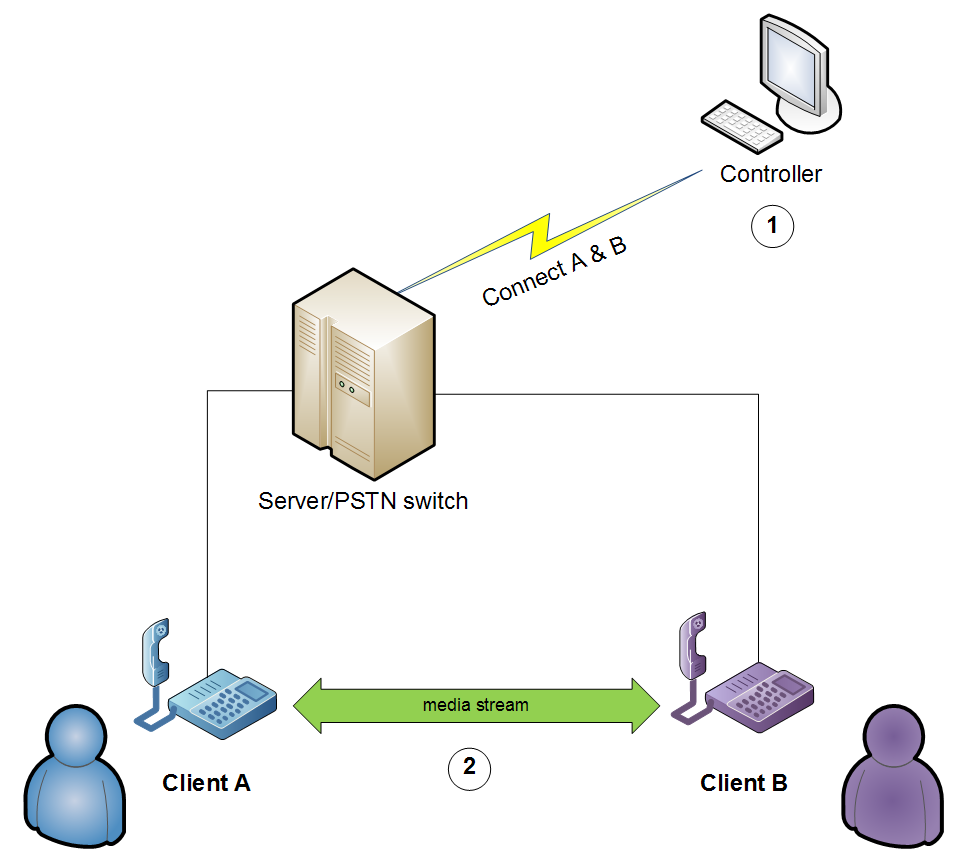
\epsfig{file=chap03/resources/3pcc, width=4in}
\caption{Third party call control}
\label{fig:ThirdPartyCallControl}
\end{figure}

A general work flow of 3pcc is shown in Figure \ref{fig:ThirdPartyCallControl}. The initial side of the phone is the \textit{controller}. The \textit{controller} sends a signal ``connect \textit{client \nolinebreak A} and \textit{client \nolinebreak B}'' to the server \hyperref[fig:ThirdPartyCallControl]{\ding{172}}. And the server establishes a call between \textit{client A} and \textit{B} \hyperref[fig:ThirdPartyCallControl]{\ding{173}}.


\section{Why Web Call Example Application?}
\label{sec:BackgroundStudy:WhyWebCallExampleApplication}

\textit{``Based on IMS/SIP network technology, the Web Call SDK integrates SIP call control functionality into web containers. This presents an efficient way of implementing the communication convergence of Web, IMS/SIP network, and CS networks. It does not require the installation of client-side browser plug-ins or special client software as most other VoIP services require.''} \cite{WebCallSDK}

The Web Call Example Application is neither a service provider nor a client that described above. It is more like a controller which acts as an initial side in third party call control. That is, it supports all standard client and service provider. Another advantage of Web Call Example Application is that desktop browser view, mobile browser view and Java ME client all share a same database. The user can access a same contact book and use a same service account from different platform. None of the solution provider or client has the same function.







% ********** End of chapter 3 **********
